\chapter{Description and Probability}

\vspace{1em}
\hfill
\begin{minipage}[c]{0.55\textwidth}
\raggedleft
\small\itshape
The fundamental problem of communication is that of reproducing at one point either exactly or approximately a message selected at another point.\\[0.5em]
\upshape\footnotesize Claude Shannon, \textit{A Mathematical Theory of Communication} (1948)
\end{minipage}%
\hspace{0.5em}
\begin{minipage}[c]{0.12\textwidth}
% \includegraphics[width=\textwidth]{figures/ch03_description.png}
\end{minipage}
\vspace{1.5em}

\noindent Suppose you have to send one of eight possible messages to a friend over a wire that transmits binary digits. Zero or one. Nothing else.

The obvious encoding is three bits per message. Eight messages, $2^3 = 8$ codes, one per message. Each transmission costs three bits.

Now suppose the messages are not equally common. Half the time you want to send message A. The rest is split among the other seven. Is three bits per message still the best you can do?

No. You can do better by using shorter codes for common messages and longer codes for rare ones. The average length drops below three bits.

This chapter is about that idea, taken seriously. The conclusion is that description length and probability are not separate things. They are the same structure seen from two sides. In the next chapter, this conclusion fills the hole that Chapter 2 left in the foundations of Bayesian inference.

\section*{Variable-length codes}

Let us be specific. You have four possible messages with these probabilities:

\begin{itemize}
\item Message A: probability $1/2$
\item Message B: probability $1/4$
\item Message C: probability $1/8$
\item Message D: probability $1/8$
\end{itemize}

The fixed-length code uses two bits per message: A $=$ 00, B $=$ 01, C $=$ 10, D $=$ 11. Average length: two bits.

Try a variable-length code: A $=$ 0, B $=$ 10, C $=$ 110, D $=$ 111. Average length:

$$\tfrac{1}{2}(1) + \tfrac{1}{4}(2) + \tfrac{1}{8}(3) + \tfrac{1}{8}(3) = 0.5 + 0.5 + 0.375 + 0.375 = 1.75 \text{ bits}.$$

A quarter of a bit per message saved, on average. Over many messages, this is real.

But there is a catch.

\section*{The decoding problem}

Variable-length codes have a subtle hazard. Suppose your friend has been receiving bits, and they see:

$$0110100\ldots$$

Where does each codeword end? Could ``0'' be a complete code for A, with ``110'' following as the code for C? Or could ``01'' be a partial code that pairs with later bits to make something else?

If two codewords could be read as starting the same way, you cannot tell them apart on a wire that does not send pauses.

In the example above, the code $A=0$, $B=10$, $C=110$, $D=111$ has a special property: no codeword is a prefix of another. So when your friend sees a ``0'', they know that is the entire A code. When they see a ``1'', they know to keep reading until they see one of $10$, $110$, $111$.

A code with this property is called \emph{prefix-free}: no codeword is a prefix of another. It can be decoded without delimiters.

Not every code is prefix-free. The code $A=0$, $B=01$ is not, because A's code (0) is a prefix of B's code (01). A stream beginning ``010'' is ambiguous: it could be A then 10-something, or B then 0-something. The code itself does not tell you which.

Prefix-free codes can be decoded unambiguously from a stream. They are the natural codes for self-describing data, where the code itself indicates when it has ended.

\section*{Codes as trees}

Prefix-free codes have a clean visual structure: they correspond to binary trees, where each codeword is a path from the root to a leaf. Figure~\ref{fig:prefix-tree} shows the tree for our four-message code.

\begin{figure}[h]
\centering
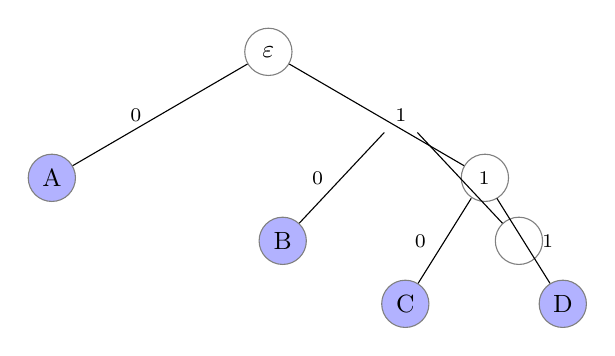
\begin{tikzpicture}[
  scale=1.0,
  every node/.style={circle, draw=gray, minimum size=6mm, font=\small, inner sep=1pt},
  level distance=1.6cm,
  level 1/.style={sibling distance=5.5cm},
  level 2/.style={sibling distance=3cm},
  level 3/.style={sibling distance=2cm}
]
  \node {$\varepsilon$}
    child {node[fill=blue!30] {A} edge from parent node[draw=none, fill=none, left, font=\scriptsize] {0}}
    child {node {} edge from parent node[draw=none, fill=none, right, font=\scriptsize] {1}
      child {node[fill=blue!30] {B} edge from parent node[draw=none, fill=none, left, font=\scriptsize] {0}}
      child {node {} edge from parent node[draw=none, fill=none, right, font=\scriptsize] {1}
        child {node[fill=blue!30] {C} edge from parent node[draw=none, fill=none, left, font=\scriptsize] {0}}
        child {node[fill=blue!30] {D} edge from parent node[draw=none, fill=none, right, font=\scriptsize] {1}}
      }
    };
\end{tikzpicture}
\caption{The prefix tree for the code $A=0$, $B=10$, $C=110$, $D=111$. Each codeword is the path from the root to a filled leaf, read off the edge labels. Empty internal nodes are prefixes that continue. The prefix-free property is automatic: codewords sit at leaves; prefixes sit at internal nodes; no codeword is also a prefix of another.}
\label{fig:prefix-tree}
\end{figure}

The root has two children. The left child is A: a complete code, a leaf. The right child is the prefix ``1'', which has its own children: ``10'' (B, a leaf) and ``11'' (a prefix that continues). The prefix ``11'' has children ``110'' (C) and ``111'' (D).

Internal nodes are prefixes that continue. Leaves are codewords. The prefix-free property is automatic.

This structure is universal. Every prefix-free binary code is a binary tree with codewords at the leaves. And every binary tree with codewords at the leaves is a prefix-free binary code.

\section*{Kraft's inequality}

A key question: which sets of codeword lengths can be realized by a prefix-free code?

You cannot, for instance, have four codewords all of length one. There are only two binary strings of length one (``0'' and ``1''), so at least two of the four codewords must be longer.

You cannot have five codewords of length two. There are only four binary strings of length two.

There is a precise constraint. For any prefix-free binary code with codeword lengths $\ell_1, \ell_2, \ldots$,

$$\sum_i 2^{-\ell_i} \leq 1.$$

This is Kraft's inequality. It is the answer to the question.

Why is it true? Each codeword of length $\ell$ occupies $2^{-\ell}$ of the unit interval below the root, in the sense of Figure~\ref{fig:kraft}. A codeword of length one uses half the tree. A codeword of length two uses a quarter. A codeword of length three uses an eighth.

\begin{figure}[h]
\centering
\begin{tikzpicture}[scale=1.0]
  % Unit interval as a horizontal bar
  \draw[thick] (0, 0) rectangle (8, 0.8);

  % Slab for A (length 1, width 4)
  \fill[blue!25] (0, 0) rectangle (4, 0.8);
  \draw[thick] (4, 0) -- (4, 0.8);
  \node[font=\small] at (2, 0.4) {A: $\tfrac{1}{2}$};

  % Slab for B (length 2, width 2)
  \fill[blue!45] (4, 0) rectangle (6, 0.8);
  \draw[thick] (6, 0) -- (6, 0.8);
  \node[font=\small] at (5, 0.4) {B: $\tfrac{1}{4}$};

  % Slab for C (length 3, width 1)
  \fill[blue!65] (6, 0) rectangle (7, 0.8);
  \draw[thick] (7, 0) -- (7, 0.8);
  \node[font=\scriptsize] at (6.5, 0.4) {C: $\tfrac{1}{8}$};

  % Slab for D (length 3, width 1)
  \fill[blue!85] (7, 0) rectangle (8, 0.8);
  \node[font=\scriptsize] at (7.5, 0.4) {D: $\tfrac{1}{8}$};

  % Axis annotations
  \node[font=\scriptsize, anchor=north] at (0, -0.1) {0};
  \node[font=\scriptsize, anchor=north] at (8, -0.1) {1};

  % Total annotation
  \draw[gray, thin] (0, -0.5) -- (8, -0.5);
  \node[font=\scriptsize, gray, anchor=north] at (4, -0.55) {$\sum 2^{-\ell_i} = \tfrac{1}{2} + \tfrac{1}{4} + \tfrac{1}{8} + \tfrac{1}{8} = 1$};
\end{tikzpicture}
\caption{Kraft's inequality visualized for the code $A=0$, $B=10$, $C=110$, $D=111$. Each codeword of length $\ell$ uses $2^{-\ell}$ of the unit interval. The slabs fit exactly: $1/2 + 1/4 + 1/8 + 1/8 = 1$. The code is complete; the whole interval is used. A code with $\sum 2^{-\ell_i} < 1$ would leave gaps. A code with $\sum 2^{-\ell_i} > 1$ would not fit and could not be prefix-free.}
\label{fig:kraft}
\end{figure}

In a prefix-free code, codewords cannot share full paths from root to leaf. Each leaf belongs to exactly one codeword. So the regions assigned to codewords do not overlap, and their total cannot exceed one.

For our four-message code, the lengths are $1, 2, 3, 3$. The Kraft sum is

$$2^{-1} + 2^{-2} + 2^{-3} + 2^{-3} = 1.$$

Exactly one. The code is \emph{complete}: every leaf in the tree is a codeword.

Any set of codeword lengths with $\sum 2^{-\ell_i} \leq 1$ admits a prefix-free code. Any set with $\sum 2^{-\ell_i} > 1$ does not. The arithmetic is the only constraint.

\section*{The bridge}

Now the connection to probability.

Take any prefix-free code with lengths $\ell_1, \ell_2, \ldots$ satisfying Kraft. The values $2^{-\ell_i}$ are nonnegative and sum to at most one. After normalizing (if the sum is less than one), they are a probability distribution:

$$P(i) = \frac{2^{-\ell_i}}{\sum_j 2^{-\ell_j}}.$$

For a complete code, the sum is already one and the normalizer is unnecessary: $P(i) = 2^{-\ell_i}$.

So every prefix-free code defines a probability distribution. Shorter codewords correspond to higher probabilities; longer codewords to lower.

The converse also holds. Given any probability distribution $P$ over a countable set of messages, there is a prefix-free code with lengths $\ell_i$ close to $-\log_2 P(i)$. The approximation comes from $\ell_i$ being an integer; the underlying logarithm is real-valued. Shannon and Fano gave a recipe in the 1940s. Huffman gave an optimal one in 1952.

So every probability distribution gives a prefix-free code, and every prefix-free code gives a probability distribution. The two are interconvertible. Description length and probability are the same structure seen from two sides.

The relationship has a name: a prefix-free code and a probability distribution related by $\ell_i \approx -\log_2 P(i)$ are said to be \emph{coupled}. Codes are descriptions; probabilities are weights. Coupling means the description length is approximately the negative logarithm of the weight, and the weight is two to the negative description length.

\section*{What this gets us}

The bridge does several things at once.

It tells us \emph{shorter descriptions are more probable}, not by stipulation but by structural correspondence. If you have a way of describing something in few bits, the weight that gets attached to that thing is the same weight the code-as-probability scheme implies.

It tells us \emph{any description scheme implies a prior}. Choose a description language (English, binary, computer programs in some language). Choose a way to assign lengths. By the bridge, you have a probability distribution over things being described.

It tells us \emph{the choice of description language matters, but is constrained}. Different languages give different lengths and therefore different priors, but every language must respect Kraft. The arithmetic does not permit a description scheme that disagrees with itself.

The catch: this does not yet pick out a single description language. Different languages give different priors. To get a unique prior, we need a special description language. One that has a claim to universality.

\section*{Where this leaves you}

Description length and probability are coupled by Kraft's inequality. Shorter descriptions correspond to higher probabilities. Any description scheme implies a prior; any prior implies a description scheme.

The next chapter chooses the description language: computer programs. The choice has a strong claim to universality, because any reasonable computational system can be simulated by any other up to a constant. This is what the \emph{universal} in ``universal prior'' refers to.

Chapter 4 also stretches the picture in a direction this chapter did not: from finite codes for known messages to infinite codes for messages that include unbounded structure. Solomonoff's prior is what you get when you take Kraft seriously for the most general possible description language.

That is where the prior problem closes.
